\documentclass{elteikthesis}

\usepackage[utf8x]{inputenc}
\usepackage[english,hungarian]{babel}
\usepackage{amssymb}
\usepackage{pgfplots}

\selectlanguage{hungarian}

\title{Függvény interpoláció megjelenítése}
\author{Szitár Gergő}
\supervisor{Dr. Krebsz Anna}
\supervisorstitle{egyetemi docens}
\period{Programtervező Informatikus BSc}
\thesisyear{2016}
\department{Numerikus Analízis tanszék}

\begin{document}

\frontmatter

	\maketitle
	\tableofcontents
	
\mainmatter

\chapter{Bevezetés}
\paragraph{}
A matematika segítségével változásokat, folyamatokat, tulajdonságokat megpróbáljuk függvények segítségével leírni, azonban a bonyolult függvények kiszámítása nagyon költséges, polinom interpolációval egy közeli becslést tudunk kapni kisebb műveletigénnyel. Ilyenkor megpróbálunk közelíteni az eredeti függvényhez, ezt a módszert hívjuk interpolációnak.
\paragraph{}
A lényege, hogy mérések, mintavételezések segítségével bizonyos pontokban meghatározzuk a függvény értékét, és ezen eredmények segítségével készítünk egy olyan függvényt, mely áthalad ezeken a pontokon. Vagyis egy olyan $I(x)$ függvény meghatározása, melyre teljesül, hogy $I(x_i)=f(x_i)=y_i \; \forall i = 0 \dots n$, ahol az $x_0, \dots, x_n$ pontok a mérések helyeit, továbbiakban alappontokat, és $y_0, \dots, y_n$ a mérések eredményét, vagyis az alappontokban az eredeti függvény által felvett értékeket jelölik.
\paragraph{}
Az előállított közelítési függvény típusa alapján három nagyobb csoportba sorolhatjuk a módszereket
\begin{itemize}
\item Polinomiálisak, ekkor az $n+1$ darab alappontra egy $n$-ed fokú polinomot illesztünk.
\item Trigonometrikusak, ekkor $sin$ és $cos$ függvények segítségével történik az interpoláció. Periodicitásuk miatt hasznosak.
\item Racionális, ekkor két polinom hányadosaként adjuk meg a közelítést.
\end{itemize}
A továbbiakban csak a polinomiális módszerrel foglalkozunk, hiszen ezen függvényeket adott pontban lineáris időben ki tudjuk értékelni.
\paragraph{}
A mai világban minden számítógépben megtalálható egy grafikus processzor, mely a képi megjelenítést teszi lehetővé. Ezt kihasználva, a program nem csak előállítja a közelítést, hanem meg is jeleníti ezt. Egy dimenziós függvény esetében ez egy vonalat, két dimenziós esetén egy felszínt jelent.
\paragraph{}
Ehhez szükségünk van a létrejött függvényt véges sok pontban kiszámolnunk, a lineáris idejű kiértékelés biztosítja, hogy egy nem túl nagy fokszámú polinomot is viszonylag gyorsan meg tudjunk jeleníteni. Ezután a felhasználó már vizualizálva láthatja a függvény becslését, könnyebben fellelheti az érdekes, további vizsgálatot megkövetelő részeket. Ilyenek lehetnek a szélső értékek, gyökök, más függvényekkel vett metszéspontok.
\paragraph{}
Mindig is szerettem ötvözni más-más területen megszerzett tudásomat, így ebben a dolgozatban is ez a célom. A vizualizáció mindig is érdekelt, így a megjelenítés már adott volt. A matematikai háttér kisebb utána olvasás és kutatás után véglegesedett ki, hiszen az egyetem alatt csak egyváltozós függvények interpolációját tanultuk, de találtam módszereket az interpolációs polinom előállítására többváltozós függvények esetén. A matematikai függvényeket leíró formális nyelv átalakítása kiértékelhető formára hasonló elven működik, mint a fordítóprogramok működése. Így végül egy viszonylag komplex és sokrétegű programmal sikerült megoldani a kitűzött feladatot. További érdekes információkat a Tudományos háttér című fejezetben találhatnak, ahol részletes leírás található az egyes témakörökből.

\chapter{Tudományos háttér}
\section{Interpoláció}
\paragraph{}
A program polinom interpoláció felhasználásával készíti el a közelítést. Célja, hogy $n+1$ darab pontra egy $n$-ed fokú polinomot illesszen. Ezen függvények előnye, hogy kiszámításuk viszonylag olcsó, a Horner algoritmus felhasználásával lineáris időben ki lehet őket értékelni. Lentebb a két legnépszerűbb interpolációs polinom előállítását mutatom be. 
\subsection{Lagrange-interpoláció}
\paragraph{}
A módszer lényege, hogy $n+1$ darab különböző alappontból előállítunk egy polinom bázist, melyeket Lagrange alappolinomoknak nevezünk, és a lineáris kombinációjukkal előállítjuk a közelítő függvényt. Előnye a módszernek, hogy könnyen bővíthető több dimenzióra is, hátránya a függvény kiértékelés magas költsége.
\paragraph{}
A bázis előállításához két követelményünk van:
\begin{itemize}
\item A $k$-adik bázis az $x_k$ alappontban 1 értéket vegyen fel.
\item A $k$-adik bázis az $x_i, i \neq k$ alappontokban pedig 0 értéket vegyen fel.
\end{itemize}
Formálisan felírva:
$$
l_i(x_j) =
\left\{
  \begin{array}{lr}
    0 & : i \neq j\\
    1 & : i = j
  \end{array}
\right.
\quad \forall i = 0 \dots n
$$
Így egy olyan $n$ fokú polinomot kell előállítanunk, melynek ismerjük a gyökeit. Fel tudjuk írni a polinomot gyöktényezős alakban.
$$
(x-x_0)\cdot(x-x_1)\cdots(x-x_{i-1})\cdot(x-x_{i+1})\cdots(x-x_n)
$$
Ezzel az első feltételt sikerült teljesíteni, ám az $x_i$ pontban felvett értéke még nem 1, ezért le kell osztanunk az ebben a pontban felvett értékkel.
$$
(x_i-x_0)\cdot(x_i-x_1)\cdots(x_i-x_{i-1})\cdot(x_i-x_{i+1})\cdots(x_i-x_n)
$$
Sikerült is megkonstruálnunk azokat a bázis polinomokat, melyek megfelelnek a feltételeinknek. Kisebb átalakításokkal könnyen szorzat formára tudjuk hozni:
$$
l_i(x) = \prod_{j = 0, j \neq i}^{n} \frac{x-x_j}{x_i-x_j}
$$
\begin{center}
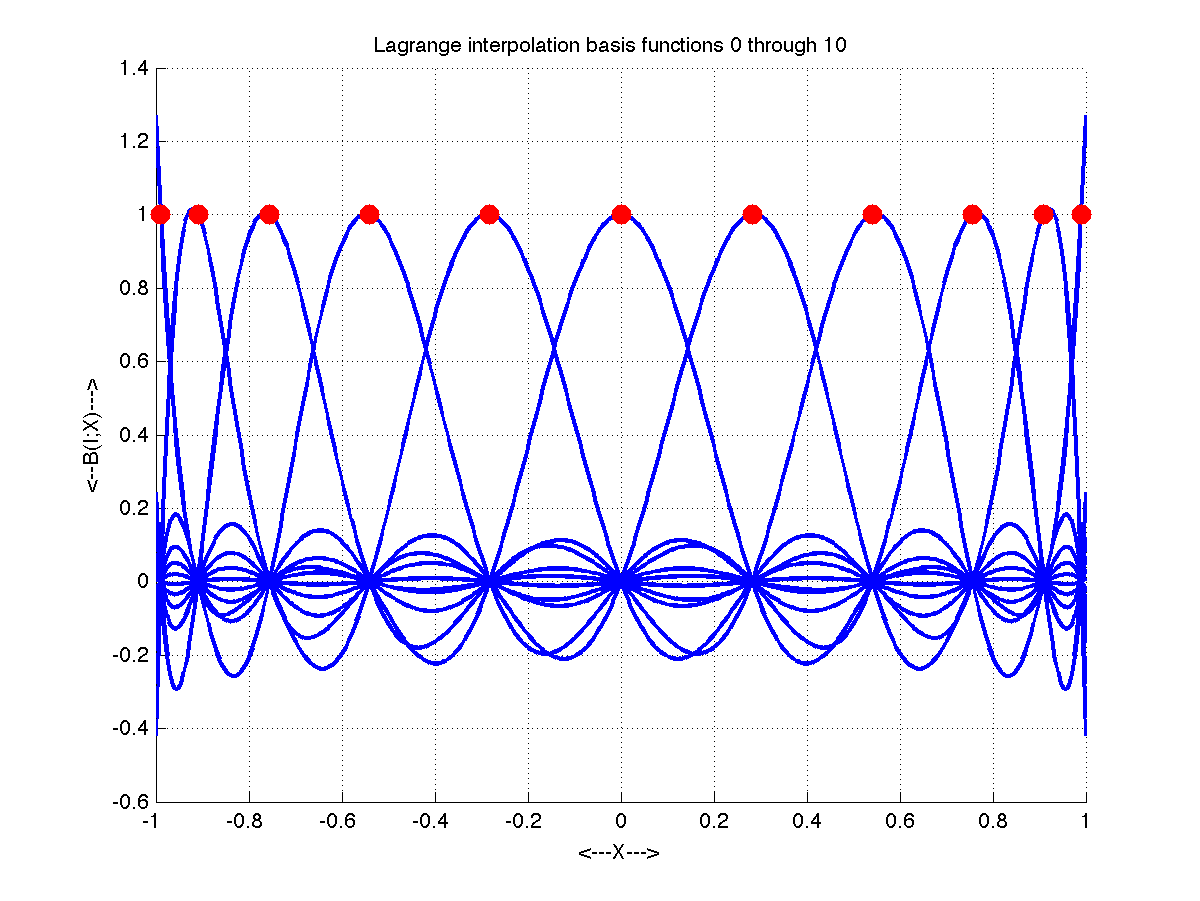
\includegraphics[width=8cm,height=6cm]{pics/lagrange_basis}\\
{\footnotesize A bázispolinomok ábrázolva.}
\end{center}
\paragraph{}
Felhasználva az előbb készített bázist, és a függvény értékeket, az alábbi interpolációs polinomot tudjuk előállítani:$$L(x) = \sum_{i=0}^{n} y_i \cdot l_i(x)$$
\begin{center}
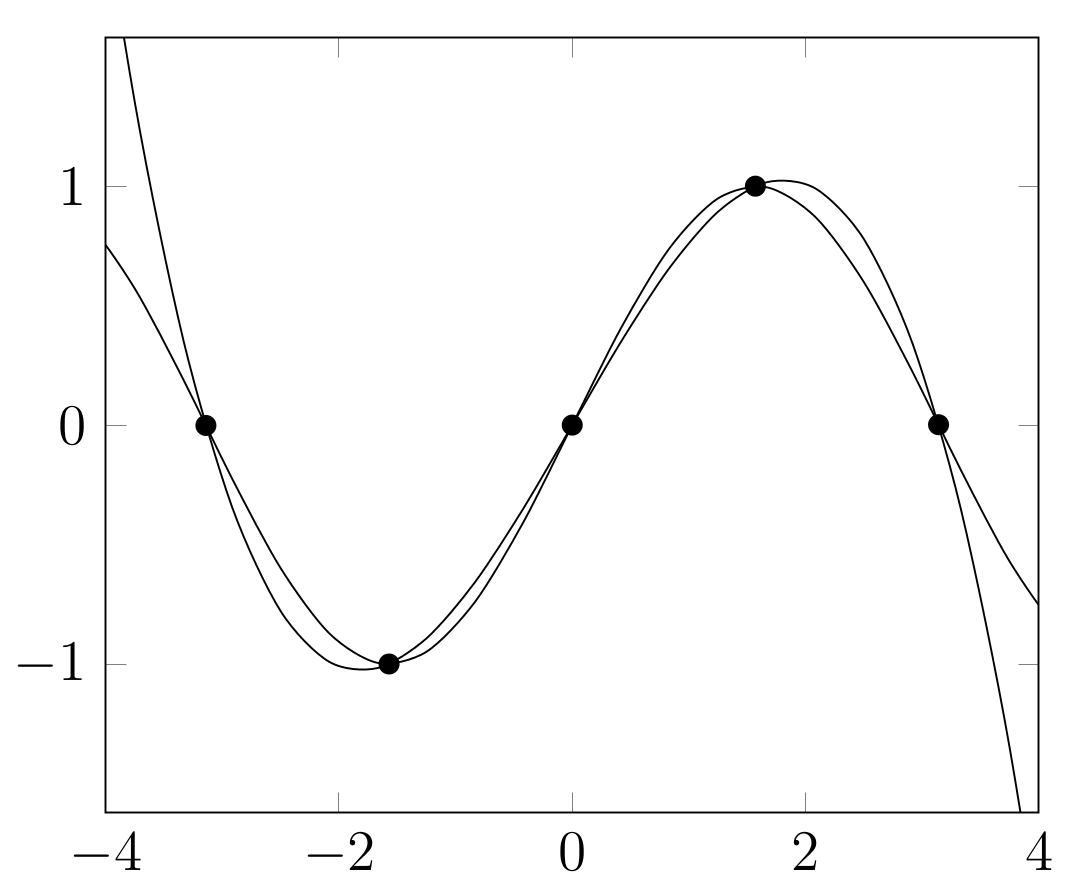
\includegraphics[width=8cm,height=6cm]{pics/polynomial_interpolation}\\
{\footnotesize Az interpolációs polinom és a függvény viszonya.}
\end{center}
\paragraph{}
Könnyen látható, hogy a fenti polinom teljesíti az interpolációs feltevést.
$$L
(x_i) = f(x_i) = y_i \quad \forall i = 0\dots{n}
$$
Az interpolációs feltétel az $x_i$ pontban az, hogy
$$
P(x_i)=\sum_{j=0}^{n} y_j\cdot l_j(x_i) = y_i
$$
Kiemelve a $j = i$ esetet a kapjuk, az alábbi alakot
$$
y_i \cdot l_i(x_i) + \sum_{j=0, i \neq j}^{n} y_j \cdot l_j(x_i)
$$
Az $l_i(x)$ függvény készítésekor feltettük, hogy az $i$-edik alappontban az értéke legyen 1, minden más pontban 0. Ezt a behelyettesítést elvégezve, egy egyszerű formát kapunk. Innen triviálisan következik, hogy az interpolációs feltétel teljesül.
\paragraph{}
A fenti bázist fel tudjuk használni, hogy kiterjesszük az interpolációt kétváltozós függvényekre, egyetlen kikötés, hogy az alappontok egy rácsot alkossanak. Ez azt jelenti, hogy az x tengelyre levetítve kapjuk az $x_0, \dots, x_n$ felosztást, ugyanígy az $y$ tengelyre $y_0, \dots, y_m$. Ekkor feltétel, hogy $\forall (x_i, y_j) \; i = 0 \dots n, \; j = 0 \dots m$ pontban tudjuk a függvény értékét. Innen az egy változónál használt elvet követve, készítünk $(n+1) \cdot (m+1)$ darab bázist, melyek lineáris kombinációja fogja megadni az eredeti függvényt.
\begin{center}
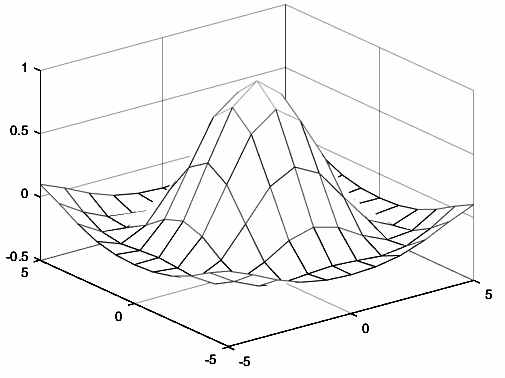
\includegraphics[width=10cm]{pics/bivariable_grid}\\
{\footnotesize Mintavételezés rácspontokban.}
\end{center}
\paragraph{}
Olyan bázist keresünk, melyekkel fel tudjuk írni az interpolációs polinomot az alábbi formában.
$$
L(x, y) = \sum_{i=0}^{n}\sum_{j=0}^{m}f(x_i, y_j) \cdot l_{i, j}(x, y)
$$
Az $l_{i, j}(x,y)$ bázis elkészítéséhez fel tudjuk használni a már egy változónál elkészített bázis polinomokat. Legyen
$$
p_i(x) = \prod_{k = 0, k \neq i}^{n}\frac{x-x_k}{x_i-x_k},\; q_j(y) = \prod_{k = 0, k \neq j}^{n}\frac{y-y_k}{y_j-y_k}
$$
A szorzatukból előáll a keresett bázis, hiszen az $l_{i, j}(x,y) = p_i(x)\cdot q_j(y)$ függvény az $(x_i, y_j)$ alappontban 1 értéket vesz fel, míg más alappontokban 0-át.
\subsection{Newton-féle interpolációs polinom}
\paragraph{}
Ez a módszer is, a Lagrange-interpolációhoz hasonlóan, egy polinom bázis lineáris kombinációjának segítségével alkotja meg a közelítést, viszont az együtthatók már nem a függvény értékek, hanem a belőlük előállított osztott differenciák lesznek. Előnye a gyors számítás, az osztott differenciák akár helyben is számolhatóak, új pont megadásakor nem kell teljesen újra számolni, elegendő csak az utolsó együtthatót kiszámolni. Hátránya, hogy nehezen terjeszthető ki több dimenzióra.
\paragraph{}
Először definiálnunk kell az osztott differenciát, $k$ darab pont osztott differenciájának a jelölése: $[y_0, \dots, y_{k-1}]$. Legyenek $x_0, \dots, x_n$ alappontok és $y_0, \dots, y_n$ értékek. Egy pontra az osztott differencia értéke önmaga, vagyis $[y_k] := y_k$. Kettő vagy több pont esetén rekurzívan számoljuk ki:
$$
[y_i, \dots, y_{i+j}] := \frac{[y_{i+1}, \dots, y_{i+j}] - [y_{i}, \dots, y_{i+j-1}]}{x_{j+i} - x_i}
$$
A továbbiakban egy egyszerűbb jelölést vezetünk be abban az esetben, ha $y_i = f(x_i)$. Ekkor $[y_0, \dots, y_{k-1}]$ helyett $f[x_0, \dots, x_{k-1}]$ használható.
\begin{center}
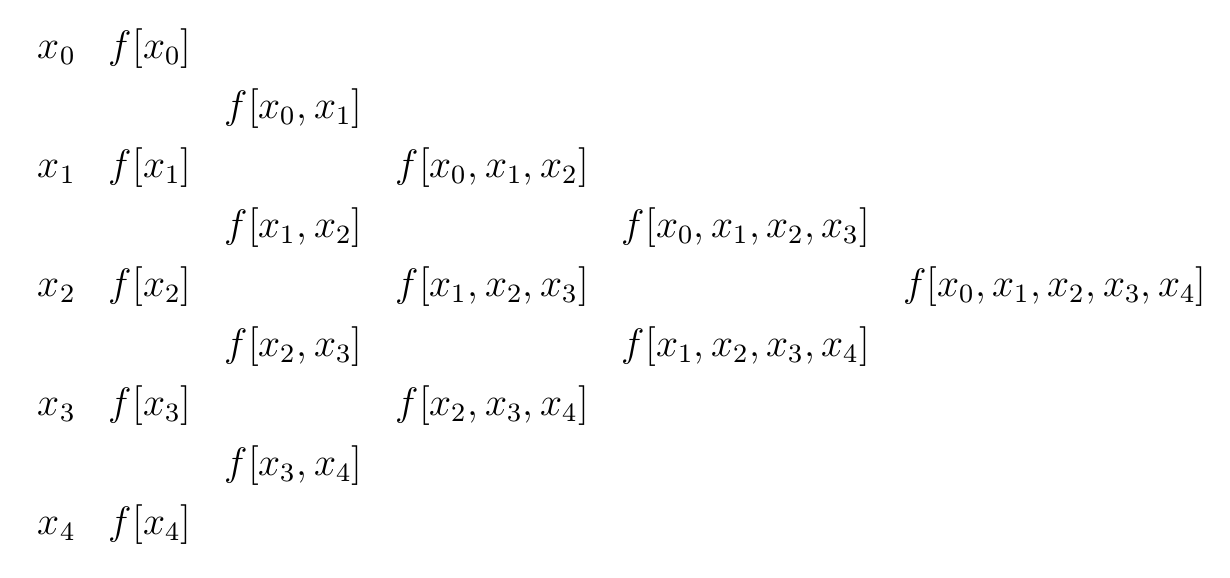
\includegraphics[width=10cm]{pics/divide_difference_table}\\
{\footnotesize Osztott differenciák táblázata.}
\end{center}
\paragraph{}
A bázis Lagrange módszerrel ellenkezően sokkal egyszerűbben felírható. Most a célunk egy könnyen bővíthető polinom bázis előállítása. Válasszuk az alábbi bázist.
$$
n_i = \prod_{j = 0}^{i-1}(x-x_j) \quad i \in [0, n]
$$
Ekkor felhasználva az osztott differenciát felírhatjuk az interpolációs polinomot egyszerű formában.
$$
N(x) = \sum_{j=0}^{n}a_j \cdot n_j(x), \quad \mbox{ahol} \; a_j = [y_0, \dots ,y_j]
$$
\subsection{Alappontok}
\paragraph{}
Mivel adott $n+1$ darab pontra egyértelműen fel lehet írni egy $n$ fokú polinomot, ezért más technikához kell folyamodnunk, ha szeretnénk csökkenteni a becslésünk hibáját. Egy bevált módszer, ha az alappontok megválasztásával próbáljuk csökkenteni a hibát.
\paragraph{}
Vegyünk egy tetszőleges $f \in [a,b]^{n+1}$ függvényt, és közelítsük egy polinommal. Legyenek az alappontok $x_0, \dots, x_n$, ilyenkor egy tetszőleges belső pontban meg tudjuk becsülni a hibát.
$$
|f(x) - I_n(x)| \leq \frac{M_{n+1}}{(n+1)!} \cdot |\omega_n(x)|
$$
$$
M_{n+1} = \max |f^{n+1}(x)| \quad x \in [a,b]
$$
$$
\omega_n(x) = (x-x_0)\cdot(x-x_1)\cdots(x-x_n)
$$
\begin{center}
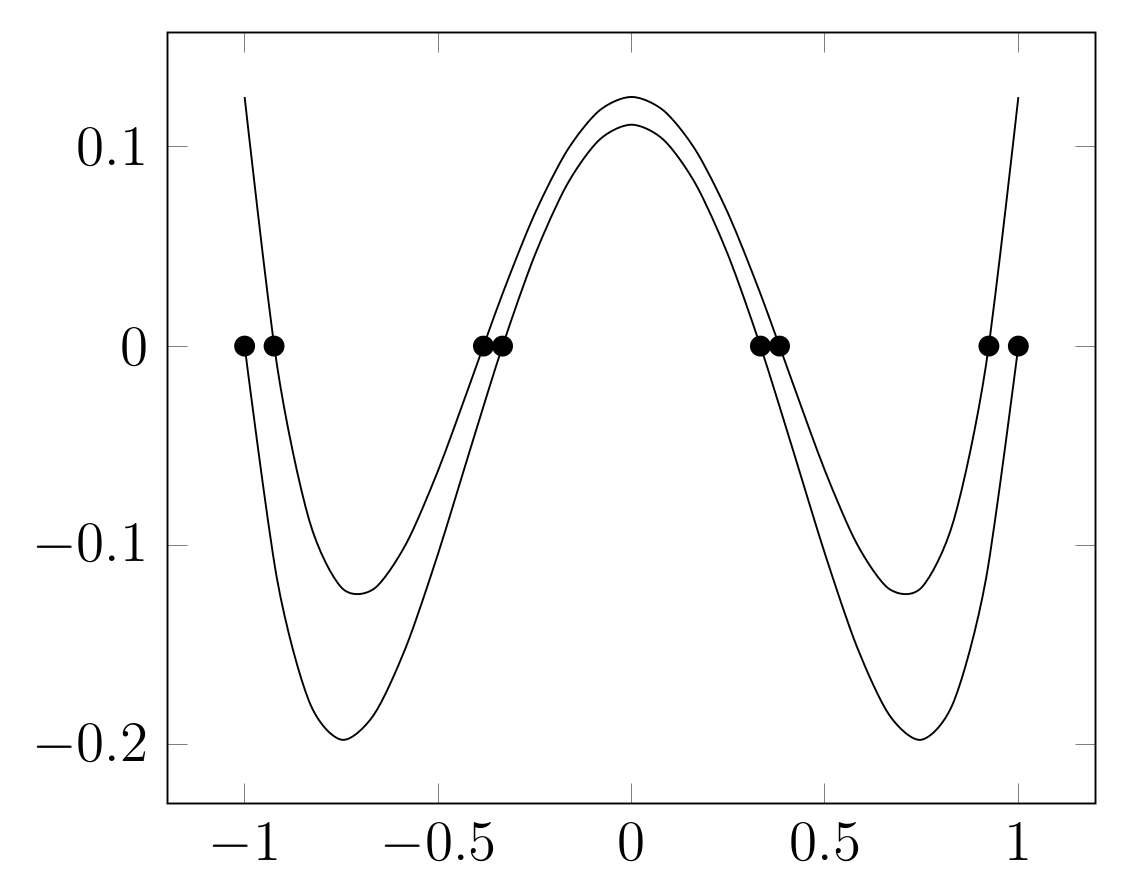
\includegraphics[width=8cm]{pics/chebyshev_and_even}\\
{\footnotesize $\omega$ függvények egyenletes és Csebisev alappontok esetén.}
\end{center}
\paragraph{}
Azonban létezik megoldás ennek a hibának a lecsökkentésére, a Csebisev alappontok használatával. A Csebisev polinomok tulajdonsága, hogy minden gyöke a $[-1,1]$ intervallumon belül helyezkedik el és az $n$-edik polinomnak $n$ darab gyöke van.
\paragraph{}
Az $n$-edik előállítása megtörténhet rekurzióval , ekkor $T_0(x)=1$, $T_1(x) = x$ és $T_n(x) = 2x \cdot T_{n-1}(x)-T_{n-2}(x)$, vagy trigonometrikus függvények segítségével $T_n(x) = cos(n \cdot arccos(x))$.
\paragraph{}
Mivel a gyökök a $[-1, 1]$ intervallumon belül vannak, ezért lineáris transzformáció segítségével tudunk megfelelő alappontokat előállítani. Az $[a,b]$ intervallumra egy $f \in [-1,1] \rightarrow [a,b]$ függvény alkalmazásával tudjuk leképezni, mely $a$ és $b$ paraméter-ek segítségével az alábbi formában áll elő:
$$
f(x) = \frac{a+b}{2}+\frac{b-a}{2} \cdot x
$$
Elértük, hogy legyen $n$ darab alappontunk az $[a,b]$ intervallumon, melyekre el tudjuk így végezni az interpolációt. Ezekkel az alappontokkal készített polinom már sokkal jobb közelítést ad.
$$
|f(x)-I_n(x)| \leq \frac{M_{n+1}\cdot(b-a)^{n+1}}{(n+1)! \cdot 2^{2n+1}}
$$
\paragraph{}
Ez annak a következménye, hogy $\omega_n(x)$ polinomnak a $0$-tól legkevésbé eltérő $1$ együtthatójú polinomot választjuk, mely a $T^*_n(x) = 2^{1-n} \cdot T_n(x)$. Ehhez a Csebisev polinom gyökeit kell megválasztani alappontnak. Ezen polinomok tulajdonsága, hogy $\max |T^*_n(x)| = 2^{1-n} \quad x \in [-1,1]$. Le tudjuk vezetni, hiszen $T_n(x) = cos(n*arccos(x))$, így a szélső értéke $1$ lesz, $T^*_n(x)$ szélsőértéke pedig $2^{1-n}$.
Már csak a fenti $[-1,1] \rightarrow [a,b]$ transzformációt kell elvégeznünk, és az eredeti hibaképletben lévő $|\omega_n(x)|$ helyére behelyettesítve megkapjuk a fenti képletet.
\newpage
\section{3D grafika}
A kezdeti számítógépek csak szöveges formában kommunikáltak a felhasználókkal, majd később született meg a grafikus ábrázolás, ami nagyban megkönnyítette a használatot. Ahogy fejlődtek a számítógépek, az egyre erősebb grafikus processzorok képesek már háromdimenziós ábrázolásra is. Ez nem tényleges háromdimenziós megjelenítést jelent, a legtöbb esetben egy három dimenziós jelenet egy adott pontból látható képét jeleníti meg.
\subsection{Modellek}
\paragraph{}
A pontábrázolás legelterjedtebb módszer a Descartes-féle koordináta-rendszer, melyben kitüntetett szerepe van az origónak, a rendszer középpontjának. Minden más $n$ darab bázis lineáris kombinációjának segítségével adható meg. Az alapértelmezett jelölésben:
$$
O = \left( \begin{array}{c} 0\\ 1\\ 0 \end{array} \right)
$$
A három bázis pedig:
$$
\mathbf{i} = \left( \begin{array}{c} 1\\ 0\\ 0 \end{array} \right) \quad \mathbf{j} = \left( \begin{array}{c} 0\\ 1\\ 0 \end{array} \right) \quad \mathbf{k} = \left( \begin{array}{c} 0\\ 0\\ 1 \end{array} \right)
$$
Ekkor a $P = (2, 1, 4)$ pontot a $\mathbf{p} = 2 \mathbf{i} + 1 \mathbf{j} + 4 \mathbf{k}$ vektor írja le.
\paragraph{}
A Polárkoordináta-rendszer esetében kitüntetett szerepe van egy alappontnak, valamint két iránynak, egységvektorok. Ekkor a pontokat az alapponttól vett távolság, és az iránytengelyekkel bezárt szög segítségével adjuk meg. Legismertebb alkalmazási területe a GPS rendszerek, ahol a Föld középpontja az alappont, a két szög pedig a földrajzi szélesség és a hosszúság.
\paragraph{}
Mivel mindkét rendszer a háromdimenziós teret írja le, ugyanazokat a pontokat, így transzformációval páronként egymáshoz tudjuk rendelni őket.
Gömbkoordináta, vagyis háromdimenziós polárkoordináta rendszerből Descartes-féle koordináta-rendszerbe az alábbi $(\mathbb{R} \times \mathbb{R} \times \mathbb{R}) \rightarrow (\mathbb{R} \times \mathbb{R} \times \mathbb{R})$ függvény segítségével tudjuk transzformálni a pontjainkat.
$$
\left( \begin{array}{c}
	R \\
	\theta \\
	\phi \end{array}
\right)
\rightarrow
\left( \begin{array}{c}
	R \cdot \sin \theta \cdot \cos \phi \\
	R \cdot \sin \theta \cdot \sin \phi \\
	R \cdot \cos \theta
\end{array} \right)
$$
Természetesen a másik irányba is létezik egy $(\mathbb{R} \times \mathbb{R} \times \mathbb{R}) \rightarrow (\mathbb{R} \times \mathbb{R} \times \mathbb{R})$, így a Gömbkoordináta rendszerbeli pontjainknak tudunk egy Descartes-féle koordináta-rendszerbeli pontot megfeleltetni.
$$
\left( \begin{array}{c}
	x \\
	y \\
	z \end{array}
\right)
\rightarrow
\left( \begin{array}{c}
	\sqrt{x^2+y^2+z^2} \\
	\arccos{\frac{z}{\sqrt{x^2+y^2+z^2}}} \\
	\arccos{\frac{x}{\sqrt{x^2+y^2}}}
\end{array} \right)
$$
A továbbiakban csak a Descartes-féle koordináta-rendszert használjuk, mert a használt alkalmazásprogramozási interfész, röviden API, szintén ezt használja.
\paragraph{}
Programozásnál sokszor használunk közelítést, ez történik a modellezés esetén is, az alakzatokat poligonok segítségével közelítjük, melyeket könnyen tudunk tárolni, pontok és köztük futó élek segítségével. Azonban ezeket az alakzatokat el is kell helyeznünk a térben, a megfelelő állapotban, ehhez pedig szükségünk van arra, hogy eltoljuk, átméretezzük és elforgassuk őket. Ezeket a transzformációkat egy mátrixszorzásnak feleltetjük meg, így sok pontra is gyorsan el tudjuk őket végezni.
\paragraph{}
Az eltolás lényege, hogy egy $P = (x_1, y_1, z_1)$ pontot egy adott $\mathbf{d} = (d_x, d_y, d_z)$ vektorral eltoljuk, és kapjuk a $P' = (x_2, y_2, z_2) = P + \mathbf{d}$ pontot. Ezt a transzformációt egy $\mathbb{R}^{4\times4}$ mátrix segítségével tudjuk végrehajtani, azonban a művelet végrehajtása előtt, ahhoz hogy a szorzás értelmezve legyen, a $P$ pontot egy negyedik elemmel, egy egyessel is ki kell egészíteni. Így áll elő az alábbi képlet.
$$
\left( \begin{array}{cccc}
	1 & 0 & 0 & d_x \\
	0 & 1 & 0 & d_y \\
	0 & 0 & 1 & d_z \\
	0 & 0 & 0 & 1 \\
\end{array} \right)
\cdot
\left( \begin{array}{c}
	x_1 \\
	y_1 \\
	z_1 \\
	1 \end{array}
\right)
=
\left( \begin{array}{c}
	x_1 + d_x \\
	y_1 + d_y \\
	z_1 + d_z \\
	1 \end{array}
\right)
$$
\paragraph{}
Forgatáskor egy adott tengely körül egy szöggel forgatjuk el a pontokat. Elegendő csak a tengelyek körüli forgatást levezetni, ugyanis velük bármilyen másikat le tudunk írni. Első lépésként el kell tolnunk a forgástengelyt az origóba, majd két főtengely körüli forgatással a forgástengelyt a harmadik vonalába transzformáljuk, majd elvégezzük a forgatást. Aztán az első két forgatás, és az eltolás inverzét alkalmazva megkapjuk a kívánt eredményt. A főtengelyek körüli forgatások rendre a következőek:
$$
\left( \begin{array}{cccc}
	\cos\alpha & -\sin\alpha & 0 & 0 \\
	\sin\alpha & \cos\alpha & 0 & 0 \\
	0 & 0 & 1 & 0 \\
	0 & 0 & 0 & 1 \\
\end{array} \right)
\quad
\left( \begin{array}{cccc}
	\cos\alpha & 0 & \sin\alpha & 0 \\
	0 & 1 & 0 & 0 \\
	-\sin\alpha & 0 & \cos\alpha & 0 \\
	0 & 0 & 0 & 1 \\
\end{array} \right)
\quad
\left( \begin{array}{cccc}
	1 & 0 & 0 & 0 \\
	0 & \cos\alpha & -\sin\alpha & 0 \\
	0 & \sin\alpha & \cos\alpha & 0 \\
	0 & 0 & 0 & 1 \\
\end{array} \right)
$$
\paragraph{}
Szükségünk van még arra, hogy egy alakzat méretét meg tudjuk változtatni, akár azonos, akár tengelyenként különböző mértékkel. Ismét elegendő, hogy az origóban lévő alakzatot méretezzük át, hiszen eltolással oda és vissza tudjuk helyezni.  Az eddigiekhez hasonlóan, ezt is feltudjuk írni egy $4 \times 4$-es mátrix formájában.
$$
\left( \begin{array}{cccc}
	s_x & 0 & 0 & 0 \\
	0 & s_y & 0 & 0 \\
	0 & 0 & s_z & 0 \\
	0 & 0 & 0 & 1 \\
\end{array} \right)
$$
\paragraph{}
Mivel minden transzformáció mátrixa azonos méretű, így könnyen tudjuk őket egymás után végrehajtani, valamint akár komplex transzformációt is létre tudunk hozni, a megfelelő mátrixok összeszorzásával. Amikor több transzformációt hajtunk végre egymás után, akkor azok mindig jobbról balra fognak sorban következni. Például ha szeretnénk a $P$ alakzatod a felére csökkenteni, az $X$ tengely körül elforgatni $90^{\circ}$-al, majd eltolni a $(1,5,-2)$ pontba, akkor azt a következő módon tehetjük meg:
$$
\left( \begin{array}{cccc}
	1 & 0 & 0 & 1 \\
	0 & 1 & 0 & 5 \\
	0 & 0 & 1 & -2 \\
	0 & 0 & 0 & 1 \\
\end{array} \right)
\cdot
\left( \begin{array}{cccc}
	\cos(\frac{\pi}{2}) & -\sin(\frac{\pi}{2}) & 0 & 0 \\
	\sin(\frac{\pi}{2}) & \cos(\frac{\pi}{2}) & 0 & 0 \\
	0 & 0 & 1 & 0 \\
	0 & 0 & 0 & 1 \\
\end{array} \right)
\cdot
\left( \begin{array}{cccc}
	0.5 & 0 & 0 & 0 \\
	0 & 0.5 & 0 & 0 \\
	0 & 0 & 0.5 & 0 \\
	0 & 0 & 0 & 1 \\
\end{array} \right)
\cdot
P
$$
\subsection{Megjelenítés}
\paragraph{}
Alakzatokból az fentebb ismertetett transzformációk segítségével létre tudjuk hozni a háromdimenziós jelenetet, azonban ezt még nem lehet megjeleníteni, hiszen a legtöbb számítógép kimeneti perifériája egy monitor, ami csak kétdimenziós képmegjelenítést támogat. Így csak egy térbeli hatást tudunk kelteni, például azzal, hogy a közelebbi tárgy eltakarja a távolabbit, ami messzebb van, az kisebbnek látszódik.
\paragraph{}
A továbbiakban egy összetett struktúrát, a vertexeket fogjuk használni, melyek tartalmazzák a pont koordinátáját, a színét vagy a textúra koordinátáit, esetlegesen a normálisokat. Az első komponens, koordináta, adja meg, hogy a térben hol helyezkedik el az adott pont. A pont színét vagy tudjuk, hogy a textúra és a koordináta segítségével határozzuk meg. A normálisok egy felületre, a pontok esetében arra melynek részei, merőleges vektorok. Segítségükkel tudunk fényeket, visszaverődést meghatározni.
\paragraph{}
A grafikus szerelőszalag feladata, hogy a vertexekből előállítson egy kétdimenziós képet. Mivel ez egy összetett feladat, ezért több részfeladatra bontás, és csővezeték használatával párhuzamosítható és gyorsítható.
\paragraph{}
Legelső lépés a vertexek sorba állítása a feldolgozáshoz, ezután egymás után haladnak sorban a csővezetékben. Innentől vertexenként külön-külön végrehajtódnak a különböző műveletek. A vertex-feldolgozó egység bemenete egy vertex (pozíció, szín, normális, egyebek), kimenete egy már megfelelően transzformált vertex. Megjelenítéshez szükség van három fő transzformációra, melyek mátrixszorzásként hajtódnak végre a vertex pozícióján. Az világban megfelelő helyre történő transzformálás az első, az előző részben bemutatott egyszerű transzformációk szorzataként áll általában elő. Ezután a nézet transzformáció következik, ami azt állítja be, hogy mi melyik pontból, és hogyan lássuk az elkészített jelenetet. Utolsó lépésként pedig az előállított végső jelenetet vetíti le a kétdimenziós vásznunkra. A három transzformációt elvégezve az egység továbbküldi a vertexet.
\paragraph{}
Már elkészített transzformált vertexekből háromszögeket épít fel a következő egység, azért háromszöget, mert azok biztosan egy síkon vannak, így könnyű velük dolgozni. Az elkészült háromszögekből ezután levágja azokat a részeket, melyek kilógnak a látótérből. Ügyelve arra, hogy továbbra is háromszögek maradjanak, ezért, ha levágás után négyszög keletkezne, akkor azt két háromszögre bontja fel. Az előállított síkidomok ezután további feldolgozásra haladnak tovább a szalagon.
\paragraph{}
Raszterizáció lényege, hogy az elkészült háromszögeket a lehető legkisebb egységekre bontsa. Első lépésben meghatározza egy háromszögről, hogy mely pixelek tartoznak hozzá, vagyis vannak benne. Ezután a háromszög három csúcspontjának színe és távolsága alapján meghatározza minden fragment színét, majd innen az adatokat egy bufferba küldi tovább. A kép frissítésekor a buffer tartalma alapján ki tudjuk rajzolni a képernyőre a kívánt alakzatot.
\begin{center}
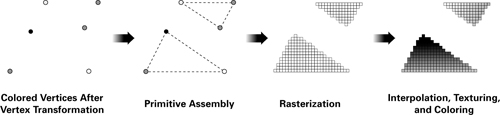
\includegraphics[width=15cm]{pics/graphic_pipeline}\\
{\footnotesize A grafikus szerelőszalag fő lépései}
\end{center}

\newpage
\section{Formális nyelvek és fordító programok}
Matematika világában mindent megpróbálunk formálisan leírni, mert csak így tudjuk őket használni és bizonyítani. A nyelvekkel is ugyanígy járunk el, megpróbálunk szabályokat felírni, mely segítségével a nyelv levezethető. Ezzel el tudjuk dönteni, hogy egy adott, formális nyelvben vett szó, egy adott nyelvhez tartozik-e. Ez a folyamat történik akkor is, mikor a fordító program az általunk írt kódot elemzi és készíti el a futtatható állományt. Ekkor a programunk lesz a szó, és a fordítóprogram különböző elemzői döntik el, hogy valóban az adott programnyelvbe tartozik-e a kódunk.
\subsection{Nyelvek leírása formálisan}
\paragraph{}
A nyelvek alapjai a szimbólumok, a nem üres véges halmazuk pedig az ábécé. Egy $L$ ábécé feletti szavak halmazát $L^+$-al jelöljük, ha az üres szót is belevesszük, akkor $L^*$-al jelöljük.
\paragraph{}
Formális nyelveket le tudunk írni nyelvtanokkal, mely megadja a nyelv ábécéjét, terminális szimbólumok, és azokat a szabályokat, melyek segítségével az adott kezdő szimbólumból el tudunk jutni a nyelv által generált összes szóig. Továbbiakban $G$ nyelvtan egy olyan négyes $(N, T, P, S)$, ahol $T$ és $N$ a terminális és nemterminális szimbólumok ábécéi, feltétel, hogy diszjunktak. $P$ a szabályok halmaza, $(N \cup T)^+ \rightarrow (N \cup T)^*$ függvények, $S \in N$ pedig a kezdőszimbólum.
\paragraph{}
Az $(X \rightarrow Y)$ szabály jelentése, hogy ha $X$-et le tudjuk vezetni, akkor $Y$-t is, ezt rekurzívan követve, ha egy szóról azt kapjuk, hogy $S$-ből levezethető, akkor a nyelv egyik szava. Könnyebb olvashatóság céljából, ha több olyan szabály létezik, mely bal oldala azonos, akkor őket össze tudjuk vonni, és a jobb oldalakat $|$-el elválasztva soroljuk fel.
\paragraph{}
Az alábbi példán az egész számokon értelmezett alapműveletek nyelvét mutatjuk be. Legyen $G=(N, T, P, S)$, ahol
$$
\begin{array}{rl}
T= & \{0, 1, 2, 3, 4, 5, 6, 7, 8, 9, +, -\} \\
N= & \{Start, Number, Digit, Operator\} \\
S= & Start \\
P= & \{Start \rightarrow Number | Number \; Operator \; Start, \\
&\; Number \rightarrow Digit | Digit \; Number, \\
&\; Digit \rightarrow 0 | 1 | 2 | 3 | 4 | 5 | 6 | 7 | 8 | 9, \\
&\; Operator \rightarrow + | -|\cdot\}
\end{array}
$$
\paragraph{}
A szabályok alkalmazásával minden szóhoz elő tudunk állítani egy szintaxisfát, melynek a gyökerében a kezdőszimbólum, a leveleiben pedig nemterminális szimbólumok állnak. Ez a fa nem minden esetben egyértelmű, léteznek olyan szavak, melyekhez több fa is tartozik. Példákban a $2+3\cdot4$ szóhoz két különböző fát tudunk előállítani, melyek később fontos szerepet töltenek be az elemzés során. Ilyenkor szükséges, hogy további elemzéshez a megfelelő fát küldjük tovább, a helyes eredmény érdekében.
\begin{center}
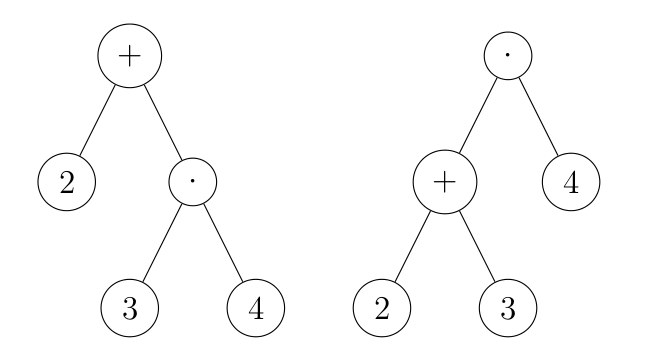
\includegraphics[width=8cm]{pics/syntax_tree}\\
{\footnotesize A $2+3\cdot4$ kifejezés két szintaxisfája.}
\end{center}
\subsection{Fordítás menete}
\paragraph{}
A fordítás első lépése a lexikális elemzés, melynek feladata, hogy a bemenetről eldöntse, megfelel a nyelv ábécéjének, és szimbólumokra, úgynevezett tokenere bontsa azt. Ennek segítségére reguláris kifejezéseket használunk, melyekkel könnyen fel tudunk írni akár bonyolultabb szimbólumokat is.
\paragraph{}
Például a $(\backslash +|-)?[0-9]+(\backslash.[0-9]+)?$ kifejezés írja le a számokat. Három rész különböztethető meg, előjel, egészrész és törtrész. Az előjelet $(\backslash+|-)?$ írja le, ahol a $+$ és $-$ az előjeleknek felel meg, a $\backslash$ az úgynevezett escape karakter, a $+$ jelnek kitüntetett jelentése van, $|$ jelöli, hogy a kettő közül az egyik, ha többet írunk egymás utána, akkor a sok közül az egyiket jelenti. Sok elem esetén listát használhatunk, $[a-z]$, ez hasonló az előzőhöz, a sok elem közül az egyikre illeszkedik. A kifejezés végén álló $?$ az előtte álló részről megengedi, hogy nullaszor vagy egyszer szerepeljen. Hozzá hasonlóan a $+$ és $*$ jelek is a mennyiséget módosítják, míg a $+$ kifejezés egyszer vagy többször, addig a $*$ megengedi, hogy egyszer sem szerepeljen. A kifejezés $[0-9]+$ része a pozitív egész számokat írja le, az utolsó része pedig, hogy a pont után másik egész szám áll.
\paragraph{}
Miután a bemenetet tokenekre bontottuk, meg kell őket feleltetnünk a $P$ halmazban szereplő szabályoknak. A szabályok alkalmazása mentén előállítjuk a szintaxis fát, amennyiben az adott bemenet a nyelv egy szava.
\paragraph{}
Szemantikus elemzést azért végzünk, hogy az elkészített grammatika egyszerűbb legyen, és egyéb olyan feladatokat teljesítsen, melyeket szükséges elvégezni, de a szintaktikus elemzéskor nem volt rá lehetőségünk. Ez tipikusan kifejezések típusának helyességének ellenőrzése, újra deklarálás, vagy a nem deklarált változók felismerése. Ezek egyszerű ellenőrzésének érdekében bevezetjük a szimbólumtáblát, mely feladata, hogy számon tartsa, mely függvények, változók vannak jelenleg definiálva, és mi az ő típusuk.
\paragraph{}
A lexikális, szintaktikus és szemantikus elemzés után már biztosítva van, hogy a fordítás lehetséges, ilyenkor az adott nyelvünket bizonyos szabályok alapján egy másik nyelvre tudjuk fordítani, mely lehet akár már futtatható kód, vagy még csak egy köztes nyelv, amiből egy másik fordítóprogram segítségével futtatható kódot kapunk.
\subsection{Matematikai függvények formális nyelve}
\paragraph{}
A függvények interpolációjához szükségünk van arra, hogy a programban a matematikai függvényeket feltudjuk ismerni, kitudjuk értékelni. Erre az előbb bemutatott formális nyelv modellt használjuk fel. Jelölje a $G=(N, T, P, S)$ a matematikai függvények nyelvét, már csak az egyes részeket kell definiálnunk.
\paragraph{}
Az ábécénk most tokenekből fog állni, melyekre illeszkedő reguláris kifejezéseket adunk meg.
$$
T=\{var, num, open, close, add, min, mul, div, pow, abs, sin, cos, tg, ctg\}
$$
Meg kell adnunk minden elemnek a reguláris kifejezését, azért, hogy a lexikális elemző fel tudja ismerni.
$$
\begin{array}{rlrl}
var & ::= x|y & num & ::= [0-9]+(\backslash.[0-9]+)? \\
open & ::= \backslash( & close & ::= \backslash)\\
add & ::= \backslash+ & min & ::= -\\
mul & ::= \backslash* & div & ::= \backslash\backslash\\
pow & ::= \backslash\wedge & abs & ::= abs\\
sin & ::= sin\ & cos & ::= cos\\
tg & ::= tg & ctg & ::= ctg
\end{array}
$$
Következő lépés, a szabályokban használt nemterminális szimbólumok megadása, ügyelve arra, hogy ezen halmaz metszete a terminális szimbólumok halmazával üres legyen.
$$N=\{Start, Binary, Unary, Expression\}$$
A nemterminális és terminális szimbólumok ismeretében meg tudjuk konstruálni a nyelv szabályait. Az $S=Start$ választásával, az alábbi formát ölti a nyelvtan:
$$
\begin{array}{rl}
P= & \{Start \rightarrow Expression, \\
&\; Expression \rightarrow open \; Expression \; close, \\
&\; Expression \rightarrow Binary, \\
&\; Expression \rightarrow Unary, \\
&\; Expression \rightarrow var, \\
&\; Expression \rightarrow num, \\
&\; Binary \rightarrow Expression \; add \; Expression, \\
&\; Binary \rightarrow Expression \; min \; Expression, \\
&\; Binary \rightarrow Expression \; mul \; Expression, \\
&\; Binary \rightarrow Expression \; div \; Expression, \\
&\; Binary \rightarrow Expression \; pow \; Expression, \\
&\; Unary \rightarrow min \; Expression, \\
&\; Unary \rightarrow abs \; Expression, \\
&\; Unary \rightarrow sin \; Expression, \\
&\; Unary \rightarrow cos \; Expression, \\
&\; Unary \rightarrow tg \; Expression, \\
&\; Unary \rightarrow ctg \; Expression\}
\end{array}
$$
A $var$ és $num$ tokeneket úgynevezett szemantikus értékkel is ellátjuk, itt tároljuk, hogy melyik változóról van szó, $x$ vagy $y$, illetve, hogy az adott számnak mi az értéke. A nyelvhez előre elkészített szimbólumtábla tartozik, melyben az egyes műveletek és függvények kiszámításának módja található. Megtalálható még benne az egyes bináris műveletek precedenciája, mely segít a helyes szintaxisfa előállításában.
\subsection{Precedencia elemző}
\paragraph{}
A precedenciák ismeretében fel kell építenünk a helyes szintaxisfát, lásd $2+3\cdot4$ esete, csak az egyik változata eredményezte a helyes végeredményt. Ilyen feladatnak többféle megoldása is létezik, futási idő, fa felépítések iránya és előre olvasott szimbólumok száma alapján. A programban egy LR(1) parser, a precedencia elemőzre esett a választás. Az L jelentése, hogy a bemenetet balról jobbra olvasva, visszalépés nélkül elemzi, az R jelentése, hogy jobboldali levezetést használ, vagyis a fát lentről felfelé építi fel. Az 1-es jelentése, hogy egyetlen szimbólum előreolvasása után dönti el, hogy a bemenetet kell léptetnie, vagy a jelenlegit redukálnia.
\paragraph{}
Az elemző két rekurzív függvény segítségével lett megvalósítva, az első feladata az elemi kifejezések felismerése, ezek jelen esetben lehetnek előjeles számok, változók, függvények, valamint zárolójelek közötti összetett kifejezések. Ezek felismerésére szolgál a másik rekurzív függvény, mely egy adott precedenciánál nagyobb összetartozó részeket ismeri fel. Az algoritmus implementációjáról és működéséről részletes leírás a Parser osztály című alfejezetben olvasható.
\paragraph{}
Utolsó lépés az előállított fa segítségével kiértékelni a függvényt adott pontban. A mélységi bejárás algoritmusának postorder változatával könnyen el is tudjuk ezt végezni, hiszen szülő mindig egy részkifejezés főművelete, így azt az után kell elvégezni, hogy a gyerekeiben lévő műveletet elvégeztük. Egészen addig kell rekurzívan lefelé mennünk, amíg el nem érünk egy levélhez, ahol két lehetőség van. Az első, hogy a levélben egy változó van, ekkor a szemantikus érték alapján kiválasztjuk, hogy melyik változó értékét kell behelyettesíteni, a másik lehetőség, hogy egy szám áll ott, ilyenkor csak a szemantikus értékkel számolunk tovább.

\chapter{Felhasználói dokumentáció}
\section{Telepítés}
\section{Használat}
\section{Gyakran ismételt kérdések}

\chapter{Fejlesztői dokumentáció}
\section{Tervezés}
\subsection{Feladat specifikálása}
\subsection{Felhasználói esetek}
\subsection{Grafikus felület}
\section{Program felépítése}
\section{Osztályok leírása}
\subsection{Controller osztály}
\subsection{MainView osztály}
\subsection{OpenGLView osztály}
\subsection{Model osztály}
\subsection{SymbolInfo osztály}
A szimbólumok információnak rendezett tárolására szolgál, minden, egy szimbólumhoz tartozó információt tárol, és publikus metódusokon keresztül nyújt elérést. A gyorsaság, és a felesleges másolások elkerülése érdekében mindig referenciákat ad a belső reprezentációra, azonban az adatok biztonságának érdekében ezek mind konstansok.
\begin{center}
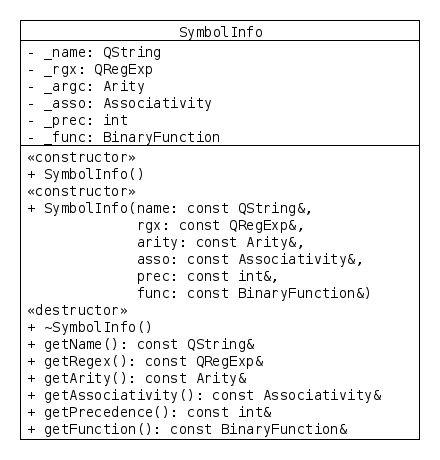
\includegraphics[width=10cm]{pics/SymbolInfo}\\
{\footnotesize A SymbolInfo osztály.}
\end{center}
\paragraph{}
A szimbólumok azonosítója a nevük, mely alapján lehet őket azonosítani. A felismeréshez szükség van egy reguláris kifejezésre, mely a bemenet elején álló kifejezést ismeri fel. Mivel különböző számú argumentuma lehet egy függvénynek, ezért az Arity enum segítéségével ezt is eltároljuk. Bináris, infix műveletek esetén szükség van a asszociativitás meghatározására is, mely a helyes műveleti sorrend előállításához szükséges. A precedencia szintén a helyes sorrendhez szükséges, azonban a különböző műveletek közötti sorrend felállításához. Az elvégzendő műveletet a függvényt is el tudjuk tárolni, így egyszerűen kiértékelhető lesz.
\section{Tesztelés}

\end{document}
